\newpage
\section{Quadratische Matrizen}
\subsection{Definition}
\textit{Quadratisch}: Matrix hat gleich viele Zeilen wie Spalten ($m=n$). \\
\textit{Hauptdiagonale}: Elemente $a_{11}, a_{22}, \dots, a_{n m}$ \\
\textit{Diagonalmatrix}: Alle Elemente unterhalb der Hauptdiagonale sind $=0$ \\
\textit{Einheitsmatrix}: Diagonalmatrix, bei der alle Diagonalelemente $=1$ sind.

\subsection{Inverse Matrizen}
\subsubsection{Definitionen}%
\label{ssub:Definitionen}
\textit{Inverses}: Matrix $A^{-1}$, für die gilt: $A \cdot A^{-1} = A^{-1} \cdot A = E$ \\
\textit{Invertierbar}: Auch \textit{regulär}. Wenn eine Matrix eine Inverse hat. Andernfalls \textit{singulär}.

\subsubsection{Inverse einer 2x2-Matrix}%
\begin{equation*}
\begin{pmatrix}
  a & b \\
  c & d
\end{pmatrix}^{-1}
= \frac{1}{ad-bc} \cdot 
\begin{pmatrix}
  d && -b \\
  -c && a
\end{pmatrix}
\end{equation*}

Um die Inverse einer grösseren Matrix $A$ zu berechnen, wendet man das Gauss-Jordan-Verfahren auf die Matrix $(A|E)$ and. Wenn $A$ invertierbar ist, führt dieses auf die Matrix $(E|A^{-1})$.

\subsection{Determinanten}
\begin{center}
  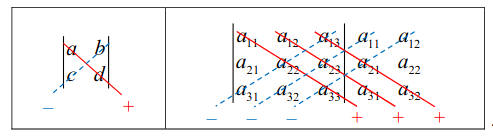
\includegraphics[width=0.7\linewidth]{images/determinante.png}
\end{center}

\subsubsection{Berechnung der Determinante einer n x n Matrix nach Laplace}%
\label{ssub:Berechnung der Determinante einer n x n Matrix nach Laplace}
\begin{enumerate}
  \item Feste Zeile oder feste Spalte wählen ($i$ oder $j$)
  \item Determinante nach folgender Formel entwickeln:
\end{enumerate}
\begin{center}
  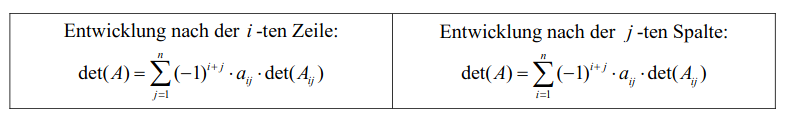
\includegraphics[width=0.7\linewidth]{images/determinante_entwickeln.png}
\end{center}
$a_{ij}$ ist das Element der Matrix $A$ der $i$-ten Zeile und $j$-ten Spalte. \\
$A_{ij}$ ist die Matrix, die man erhält, wenn man bei $A$ die $i$-te Zeile und $j$-te Spalte weglässt.

\subsubsection{Geometrische Interpretation der Determinante}%
\label{ssub:Geometrische Interpretation der Determinante}
Der Betrag der Determinante einer $2 \times 2$ Matrix ist gleich dem Flächeninhalt des Parallelogramms, das von den Spalten der Matrix (aufgefasst als Vektoren) aufgespannt wird. \\
Der Betrag der Determinante einer $3 \times 3$ Matrix ist gleich dem Volumeninhalt des Spats, das von den Spalten der Matrix (aufgefasst als Vektoren) aufgespannt wird.

\begin{center}
  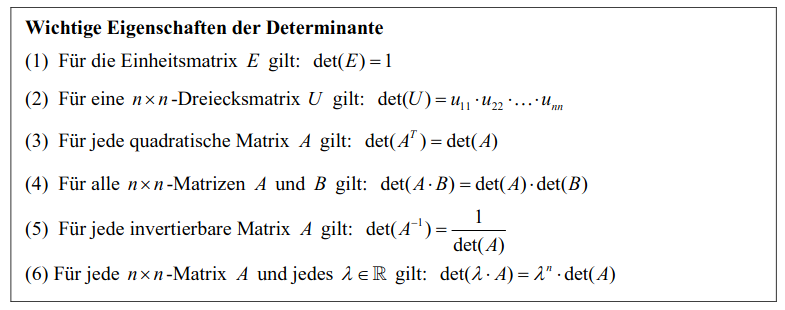
\includegraphics[width=0.9\linewidth]{images/determinante_eigenschaften.png}
\end{center}

\subsubsection{Lineare Unabhängigkeit}%
\label{ssub:Lineare Unabhängigkeit}
Vektoren $\vec{a}_1, \vec{a}_2, \dots, \vec{a}_k$ sind linear unabhängig, wenn gilt: $0 \cdot \vec{a}_1 + 0 \cdot \vec{a}_2 + \dots + 0 \cdot \vec{a}_k$ ist die einzige Linearkombination. Andernfalls sind sie linear unabhängig.

\begin{center}
  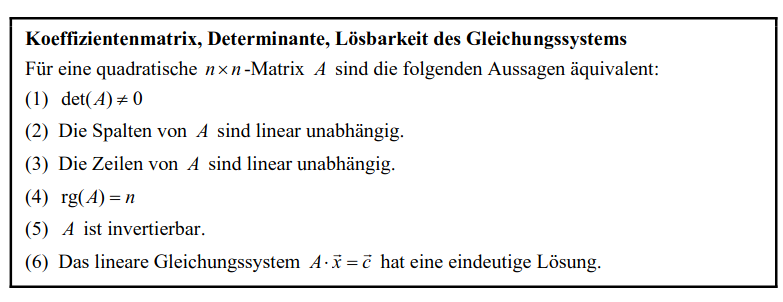
\includegraphics[width=0.9\linewidth]{images/koeffizientenmatrix.png}
\end{center}
